\documentclass[]{article}
\usepackage{lmodern}
\usepackage{amssymb,amsmath}
\usepackage{ifxetex,ifluatex}
\usepackage{fixltx2e} % provides \textsubscript
\ifnum 0\ifxetex 1\fi\ifluatex 1\fi=0 % if pdftex
  \usepackage[T1]{fontenc}
  \usepackage[utf8]{inputenc}
\else % if luatex or xelatex
  \ifxetex
    \usepackage{mathspec}
  \else
    \usepackage{fontspec}
  \fi
  \defaultfontfeatures{Ligatures=TeX,Scale=MatchLowercase}
\fi
% use upquote if available, for straight quotes in verbatim environments
\IfFileExists{upquote.sty}{\usepackage{upquote}}{}
% use microtype if available
\IfFileExists{microtype.sty}{%
\usepackage{microtype}
\UseMicrotypeSet[protrusion]{basicmath} % disable protrusion for tt fonts
}{}
\usepackage[margin=1in]{geometry}
\usepackage{hyperref}
\PassOptionsToPackage{usenames,dvipsnames}{color} % color is loaded by hyperref
\hypersetup{unicode=true,
            pdftitle={README for the performance measurement part},
            pdfauthor={Group 2},
            colorlinks=true,
            linkcolor=Maroon,
            citecolor=Blue,
            urlcolor=blue,
            breaklinks=true}
\urlstyle{same}  % don't use monospace font for urls
\usepackage{longtable,booktabs}
\usepackage{graphicx,grffile}
\makeatletter
\def\maxwidth{\ifdim\Gin@nat@width>\linewidth\linewidth\else\Gin@nat@width\fi}
\def\maxheight{\ifdim\Gin@nat@height>\textheight\textheight\else\Gin@nat@height\fi}
\makeatother
% Scale images if necessary, so that they will not overflow the page
% margins by default, and it is still possible to overwrite the defaults
% using explicit options in \includegraphics[width, height, ...]{}
\setkeys{Gin}{width=\maxwidth,height=\maxheight,keepaspectratio}
\IfFileExists{parskip.sty}{%
\usepackage{parskip}
}{% else
\setlength{\parindent}{0pt}
\setlength{\parskip}{6pt plus 2pt minus 1pt}
}
\setlength{\emergencystretch}{3em}  % prevent overfull lines
\providecommand{\tightlist}{%
  \setlength{\itemsep}{0pt}\setlength{\parskip}{0pt}}
\setcounter{secnumdepth}{0}
% Redefines (sub)paragraphs to behave more like sections
\ifx\paragraph\undefined\else
\let\oldparagraph\paragraph
\renewcommand{\paragraph}[1]{\oldparagraph{#1}\mbox{}}
\fi
\ifx\subparagraph\undefined\else
\let\oldsubparagraph\subparagraph
\renewcommand{\subparagraph}[1]{\oldsubparagraph{#1}\mbox{}}
\fi

%%% Use protect on footnotes to avoid problems with footnotes in titles
\let\rmarkdownfootnote\footnote%
\def\footnote{\protect\rmarkdownfootnote}

%%% Change title format to be more compact
\usepackage{titling}

% Create subtitle command for use in maketitle
\providecommand{\subtitle}[1]{
  \posttitle{
    \begin{center}\large#1\end{center}
    }
}

\setlength{\droptitle}{-2em}

  \title{README for the performance measurement part}
    \pretitle{\vspace{\droptitle}\centering\huge}
  \posttitle{\par}
    \author{Group 2}
    \preauthor{\centering\large\emph}
  \postauthor{\par}
      \predate{\centering\large\emph}
  \postdate{\par}
    \date{\texttt{December,\ 2nd,\ 2019}}


\begin{document}
\maketitle
\begin{abstract}
This Chapter describes the evaluation of the best sampling and model
combination, which is computed in the script `PerformanceMeasurement.R'.
\end{abstract}

\hypertarget{the-goal-of-our-performance-measurement}{%
\subsection{The goal of our performance
measurement}\label{the-goal-of-our-performance-measurement}}

After training a model it is important to check how well it performes.
Since we not only trained one model but 120 in total (6 algorithms * 5
samplings * 4 positions), it is even more important to compare all the
different models to see which one is the best. For our business case,
this means that we want to see which combination of method and sampling
we should take to predict which position, or if we even have a model,
which does it better when we leave them together.

\hypertarget{how-to-compare-the-methodsampling-combinations-for-all-positions}{%
\subsection{How to compare the method/sampling combinations for all
positions}\label{how-to-compare-the-methodsampling-combinations-for-all-positions}}

After training the models with 10-fold cross-validation, we applied them
on all the (unsampled) data from 2007 to 2013 to obtain the true
positives, true negatives, false positives and false negatives on the
training set. At the end of every model-script, we save this information
separately, to bring it all together in the script
`PerformanceMeasurement.R'. At the same time (and in the same scripts)
we also compute the testing fit on the 2014 testing data.

The first step, is to bring them all into one dataframe, to use them
easier. Then we make sure, that we used the same, unsampled data by
computing the sums of TP, TN, FP, FN, for every method/sampling/position
combination. In the CheckTibble we now see, that for every position the
whole column contains always the same number, which means this is the
case.

Then we calculate the Accuracy, Precision, Recall and the F1 score:

\[\text{Accuracy} = \frac{\text{Correct Classifications}}{\text{All Classifications}} = \frac{TP + TN}{TP+TN+FP+FN}\]
\[\text{Precision (Positice Perdictive Value)} = \frac{TP}{TP+FP}\]
\[\text{Recall (Sensitivity)} = \frac{TP}{TP+FN}\]
\[\text{F1 score (harmonic mean of precision and recall)}= 2*\frac{Precision * Recall}{Precision + Recall}\]

The result is a table showing the Accuracy, Precision, Recall and F1
scores for all the 120 model/sampling/position combination. We decided
to us the F1 score as the model estimator, because is more sensitive to
the inequality of availability of drafted vs.~undrafted players in the
target value. Therefore we just visualize the F1 score and the accuracy
of all the models for the testing set. This table is quite big, but it
is still interesting to have a look at it, to see how well which
combination performes.

\newpage

\begin{longtable}[]{@{}llrrrr@{}}
\caption{F1 score by Model/Position and Sampling on 2014 unsampled
testing data}\tabularnewline
\toprule
Method & Sampling & QB\_F1 & WR\_F1 & RB\_F1 &
Together\_F1\tabularnewline
\midrule
\endfirsthead
\toprule
Method & Sampling & QB\_F1 & WR\_F1 & RB\_F1 &
Together\_F1\tabularnewline
\midrule
\endhead
ClassificationTree & no\_sampling & 0.5161 & 0.1702 & 0.4000 &
0.2299\tabularnewline
ClassificationTree & oversampling & 0.3913 & 0.3621 & 0.3774 &
0.3280\tabularnewline
ClassificationTree & undersampling & 0.3175 & 0.3443 & 0.3385 &
0.3294\tabularnewline
ClassificationTree & Rose\_both & 0.3462 & 0.3281 & 0.2667 &
0.2814\tabularnewline
ClassificationTree & Smote & 0.3830 & 0.3559 & 0.2759 &
0.3399\tabularnewline
randomForest & no\_sampling & 0.3704 & 0.2979 & 0.4516 &
0.3619\tabularnewline
randomForest & oversampling & 0.3750 & 0.3881 & 0.3902 &
0.4122\tabularnewline
randomForest & undersampling & 0.3279 & 0.3393 & 0.3380 &
0.3443\tabularnewline
randomForest & Rose\_both & 0.4255 & 0.4043 & 0.3600 &
0.3776\tabularnewline
randomForest & Smote & 0.4211 & 0.3765 & 0.3922 & 0.3860\tabularnewline
ANN & no\_sampling & 0.6154 & 0.3860 & 0.5294 & 0.4779\tabularnewline
ANN & oversampling & 0.2857 & 0.2683 & 0.2376 & 0.2573\tabularnewline
ANN & undersampling & 0.2933 & 0.2635 & 0.2376 & 0.2683\tabularnewline
ANN & Rose\_both & 0.3056 & 0.2500 & 0.2330 & 0.2611\tabularnewline
ANN & Smote & 0.2941 & 0.2316 & 0.2286 & 0.2472\tabularnewline
KNN & no\_sampling & 0.2727 & 0.3684 & 0.2500 & 0.3636\tabularnewline
KNN & oversampling & 0.3390 & 0.2617 & 0.2222 & 0.3289\tabularnewline
KNN & undersampling & 0.3226 & 0.3878 & 0.3288 & 0.3504\tabularnewline
KNN & Rose\_both & 0.3175 & 0.2222 & 0.2169 & 0.2868\tabularnewline
KNN & Smote & 0.3636 & 0.2752 & 0.2857 & 0.3333\tabularnewline
NaiveBayes & no\_sampling & 0.4348 & 0.2812 & 0.1739 &
0.1194\tabularnewline
NaiveBayes & oversampling & 0.3279 & 0.2833 & 0.2456 &
0.2941\tabularnewline
NaiveBayes & undersampling & 0.3279 & 0.2667 & 0.3265 &
0.2737\tabularnewline
NaiveBayes & Rose\_both & 0.3571 & 0.2432 & 0.1379 &
0.2900\tabularnewline
NaiveBayes & Smote & 0.3571 & 0.2906 & 0.2667 & 0.3457\tabularnewline
LogisticRegression & no\_sampling & 0.5625 & 0.3019 & 0.5000 &
0.4522\tabularnewline
LogisticRegression & oversampling & 0.3509 & 0.3774 & 0.3200 &
0.3621\tabularnewline
LogisticRegression & undersampling & 0.3125 & 0.3495 & 0.3077 &
0.3448\tabularnewline
LogisticRegression & Rose\_both & 0.3509 & 0.3774 & 0.3288 &
0.3668\tabularnewline
LogisticRegression & Smote & 0.3333 & 0.3894 & 0.3750 &
0.3713\tabularnewline
\bottomrule
\end{longtable}

\begin{longtable}[]{@{}llrrrr@{}}
\caption{Accuracy by Model/Position and Sampling on 2014 unsampled
testing data}\tabularnewline
\toprule
Method & Sampling & QB\_Acc & WR\_Acc & RB\_Acc &
Together\_Acc\tabularnewline
\midrule
\endfirsthead
\toprule
Method & Sampling & QB\_Acc & WR\_Acc & RB\_Acc &
Together\_Acc\tabularnewline
\midrule
\endhead
ClassificationTree & no\_sampling & 0.8707 & 0.8911 & 0.9082 &
0.9000\tabularnewline
ClassificationTree & oversampling & 0.7586 & 0.7933 & 0.8316 &
0.7493\tabularnewline
ClassificationTree & undersampling & 0.6293 & 0.7765 & 0.7806 &
0.7448\tabularnewline
ClassificationTree & Rose\_both & 0.7069 & 0.7598 & 0.7194 &
0.7179\tabularnewline
ClassificationTree & Smote & 0.7500 & 0.7877 & 0.6786 &
0.7507\tabularnewline
randomForest & no\_sampling & 0.8534 & 0.9078 & 0.9133 &
0.9000\tabularnewline
randomForest & oversampling & 0.8276 & 0.8855 & 0.8724 &
0.8851\tabularnewline
randomForest & undersampling & 0.6466 & 0.7933 & 0.7602 &
0.7612\tabularnewline
randomForest & Rose\_both & 0.7672 & 0.8436 & 0.8367 &
0.8179\tabularnewline
randomForest & Smote & 0.8103 & 0.8520 & 0.8418 & 0.8433\tabularnewline
ANN & no\_sampling & 0.9138 & 0.9022 & 0.9184 & 0.9119\tabularnewline
ANN & oversampling & 0.5690 & 0.6648 & 0.6071 & 0.6209\tabularnewline
ANN & undersampling & 0.5431 & 0.6564 & 0.6071 & 0.6418\tabularnewline
ANN & Rose\_both & 0.5690 & 0.6480 & 0.5969 & 0.6284\tabularnewline
ANN & Smote & 0.5862 & 0.5922 & 0.5867 & 0.6000\tabularnewline
KNN & no\_sampling & 0.8621 & 0.9330 & 0.9388 & 0.9269\tabularnewline
KNN & oversampling & 0.6638 & 0.7793 & 0.6786 & 0.7746\tabularnewline
KNN & undersampling & 0.6379 & 0.8324 & 0.7500 & 0.7731\tabularnewline
KNN & Rose\_both & 0.6293 & 0.7067 & 0.6684 & 0.7104\tabularnewline
KNN & Smote & 0.6983 & 0.7793 & 0.7194 & 0.7672\tabularnewline
NaiveBayes & no\_sampling & 0.7759 & 0.8715 & 0.9031 &
0.9119\tabularnewline
NaiveBayes & oversampling & 0.6466 & 0.7598 & 0.7806 &
0.7851\tabularnewline
NaiveBayes & undersampling & 0.6466 & 0.7542 & 0.8316 &
0.7940\tabularnewline
NaiveBayes & Rose\_both & 0.6897 & 0.6872 & 0.8724 &
0.7881\tabularnewline
NaiveBayes & Smote & 0.6897 & 0.7682 & 0.6633 & 0.8418\tabularnewline
LogisticRegression & no\_sampling & 0.8793 & 0.8966 & 0.9082 &
0.9060\tabularnewline
LogisticRegression & oversampling & 0.6810 & 0.8156 & 0.7398 &
0.7791\tabularnewline
LogisticRegression & undersampling & 0.6207 & 0.8128 & 0.7245 &
0.7731\tabularnewline
LogisticRegression & Rose\_both & 0.6810 & 0.8156 & 0.7500 &
0.7836\tabularnewline
LogisticRegression & Smote & 0.6552 & 0.8073 & 0.7959 &
0.7776\tabularnewline
\bottomrule
\end{longtable}

We can see these two tendencies in the models:

\begin{itemize}
\tightlist
\item
  Mostly better performance with unsampled data, than with sampled data
\item
  Mostly better performance when we split the positions manually
\end{itemize}

The four following plots combine the information of both tibbles,
showing the accuracy and the F1 score on every sampling method for every
position on its own. The horizontal lines show the no information rates
for the accuracy, which displays, how a model's performance would be
when predicting only 0's.

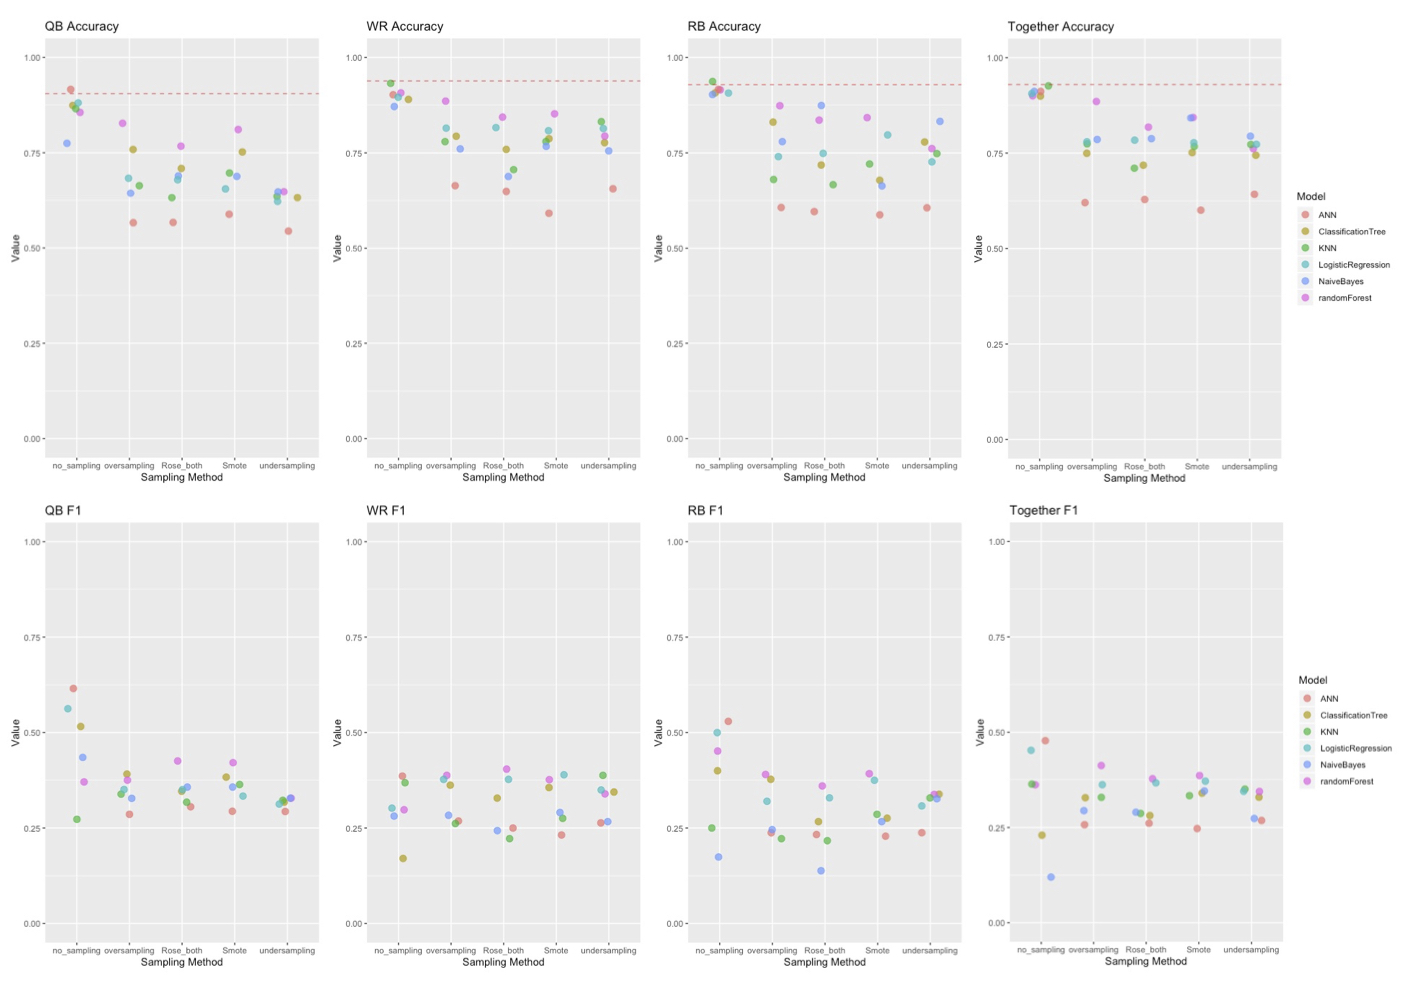
\includegraphics[width=0.95\linewidth]{Plots_8}

\newpage

\hypertarget{our-best-models}{%
\subsection{Our best models}\label{our-best-models}}

Now let's have a look at the best model/sampling combination for every
position:

\begin{longtable}[]{@{}lllrr@{}}
\caption{The best model/sampling combinations by
position}\tabularnewline
\toprule
Position & Method & Sampling & F1 & Accuracy\tabularnewline
\midrule
\endfirsthead
\toprule
Position & Method & Sampling & F1 & Accuracy\tabularnewline
\midrule
\endhead
QB & ANN & no\_sampling & 0.6154 & 0.9138\tabularnewline
WR & randomForest & Rose\_both & 0.4043 & 0.8436\tabularnewline
RB & ANN & no\_sampling & 0.5294 & 0.9184\tabularnewline
Together & ANN & no\_sampling & 0.4779 & 0.9119\tabularnewline
\bottomrule
\end{longtable}

As we see, measured at the F1-score, the atrificial neural networks
perform best for QB's, RB's and all positions together. For the WR's it
is the rose-both-sampled data trained random forest.

\hypertarget{discussion}{%
\subsection{Discussion}\label{discussion}}

Our models with accuracies up to 91.8\% seem to be very good at the
first sight. But we have to keep the reason for filtering out the
players with \textless10 played games and sampling the data in mind.
Here we applied the models to the unsampled but filtered data of 2014,
which only contains 7.01\% of drafted players. This means, that a model
predicting ``not drafted'' for every player would still perform better,
since it would still have an accuracy of 92.99\% on the whole data set
(=`Together'). In other words, our models all perform unter the `no
information rate', which makes them not really good.

Interpretations of models are always quite difficult, but the following
thoughts are pretty likely to be true, according to the TP/TN/FP/FN. Our
models are okay at predicting the likelihood of players being drafted
that didn't perform very well in college football being low. It probably
also does not too bad in predicting great players to be drafted, that
nearly must be picked (and probably are picked early in the draft). But
there must be much room for improvement for all the players that still
performed well in college, and might or might not be drafted. Again in
other words, the models can predict the more or less obvious drafts and
non-drafts but is not really better than random for the intresting
cases.

We would like to close the circle to one of our fist lessons in machine
learning, in which we were taught the following very high level formula
for models (the right part). Y denotes the true outcome (in our case
whether a player is drafted or not), f(X) is the true pattern that
describes it, and \(\epsilon\) is the noise, which appears to be random.
With our models (the left part) we try to predict a \(\hat{Y}\), which
shall be as close as possible to the true Y.

\[\hat{f}(X) = \hat{Y} \approx Y = f(X) + \varepsilon\]

Looking at this inequation we can think of three possibilities, why our
models make so many mistakes:

\begin{itemize}
\tightlist
\item
  Our models \(\hat{f_i}(X)\) do not include enough variables and/or are
  not sophisticated enough
\item
  The data is not good enough
\item
  The NFL draft contains a pretty large \(\varepsilon\)
\end{itemize}

Variables that are certainly missing in the model, are the ones that are
not quantifyable easily, such as game intelligence, strenght of the own
team, strenght of the opponents, maturity of the player and negative
factors such as criminality, drug consumation and other negative
behaviours. In the past, it happened again and again, that players with
great game statistics and a great game intelligence, which were expected
to be drafted in the first round fell far behind or were not drafted at
all, because pictures of them consuming marihuana were published.


\end{document}
